\section{Integral Theorems}
\subsection{Green's theorem}
\begin{theorem}[Green]\label{thm:Green}
    If $P = P(x, y)$ and $Q = Q(x, y)$ are continuously differentiable functions on $A \cup \partial A$ and $\partial A$ is \textit{piecewise smooth}, then
    \[
        \oint_{\partial A} P \mathrm{~d} x+Q \mathrm{~d} y=\iint_{A}\left(\frac{\partial Q}{\partial x}-\frac{\partial P}{\partial y}\right) \mathrm{d} x \mathrm{~d} y.
    \]
    Orientation of $ \partial A $ is such that $A$ lies to your left as you traverse it.
\end{theorem}
\begin{center}
    \begin{tikzpicture}
        \filldraw [color=black, thick, fill=black!20, arrow inside={end=latex',opt={black,scale=1.6}}{0,0.25,0.5,0.75}] (0,0) circle (1.5);
        \filldraw [color=black, thick, fill=white,<-] (0,0) circle (0.75);
    \end{tikzpicture}
\end{center}
\begin{note}
    It is easy to establish the result for a rectangle. Let 
    \[
        A = \{(x,y):a\le x\le b,c\le y\le d\}.
    \]
    In this case, RHS is 
    \begin{align*}
        &\int_{c}^{d} \int_{a}^{b} \frac{\partial Q}{\partial x}  \,\mathrm{d}x \,\mathrm{d}y-\int_{a}^{b} \int_{c}^{d} \frac{\partial P}{\partial y}  \,\mathrm{d}y \,\mathrm{d}x\\ 
        =& \int_{c}^{d} Q(b,y)-Q(a,y) \,\mathrm{d}y+\int_{a}^{b} P(x,c)-P(x,d) \,\mathrm{d}x\\ 
        =& \oint_{\partial A} P\dd x+Q\dd y.
    \end{align*}
    \begin{center}
        \begin{tikzpicture}
            \fill [black!20] (-2, -1) rectangle (1, 1);
            \node at (-0.5, 0) {$A$};
            \node [below] at (-1, -2) {$\dd y=0,y=c$};
            \node [above] at (0, 2) {$\dd y=0,y=d$};
            \node [right] at (2,0.5) {$ \dd x=0,x=b$};
            \node [left] at (-3,-0.5) {$ \dd x=0,x=b$};
            \draw [->-=0.5,thick] (-2, -1) -- (1, -1);
            \draw [->-=0.5,thick] (1, -1) -- (1, 1);
            \draw [->-=0.5,thick] (1, 1) -- (-2, 1);
            \draw [->-=0.5,thick] (-2, 1) -- (-2, -1);
            \draw [->] (0, 2) -- (0, 1) ;
            \draw [->] (-1, -2) -- (-1, -1);
            \draw [->] (2,0.5) -- (1,0.5);
            \draw [->] (-3,-0.5) -- (-2,-0.5);
        \end{tikzpicture}
    \end{center}
\end{note}
\begin{example}
    Let $(P, Q)=\left(-\frac{1}{2} y, \frac{1}{2} x\right) .$ Then Green's theorem tells us
    \[
    \operatorname{area}(A)=\iint_{A} \mathrm{~d} x \mathrm{~d} y=\frac{1}{2} \oint_{\partial A} x \mathrm{~d} y-y \mathrm{~d} x
    \]
    Let $A$ be the ellipse $x^{2} / a^{2}+y^{2} / b^{2} \leq 1$ so that $\partial A$ has parametrisation
    \[
    [0,2 \pi] \ni t \mapsto \begin{pmatrix}
        a \cos t \\
        b \sin t
    \end{pmatrix}
    \]
    Then
    \[
    \operatorname{area}(A)=\frac{1}{2} \int_{0}^{2 \pi}\left(a b \cos ^{2} t+a b \sin ^{2} t\right) \mathrm{d} t=\pi a b,
    \]
    as expected.
\end{example}

\subsection{Stokes' Theorem}
\begin{theorem}[Stokes]\label{thm:Stokes}
    If $ \bfF = \bfF(\bfx) $ is a continuously differentiable vector field and $S$ is an orientable piecewise regular surface with piecewise smooth boundary $ \partial  S $, then 
    \[
        \int_{S} (\curl\bfF) \cdot\mathrm{d}\mathbf{S} = \oint_{\partial S} \bfF \cdot\mathrm{d}\mathbf{x}
    \]
\end{theorem}
\begin{note}
    The ``orientable'' bit means there is a \textit{consistent} choice of normal vector at each point of $S$. i.e. $S$ has two sides. e.g. \mobius band is not orientable.
    \begin{center}
    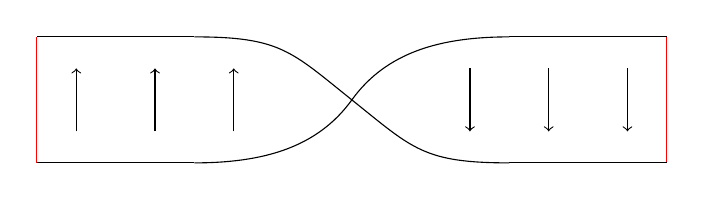
\begin{tikzpicture}[yscale=0.8]
        \node (0) at (-4, 3) {};
        \node (1) at (-4, 1) {};
        \node (2) at (4, 3) {};
        \node (3) at (4, 1) {};
        \node (4) at (2, 3) {};
        \node (5) at (2, 1) {};
        \node (6) at (-2, 3) {};
        \node (7) at (-2, 1) {};
        \node (8) at (0, 2) {};
        \node (9) at (-4, 3) {};
        \node (10) at (-3.5, 1.5) {};
        \node (11) at (-3.5, 2.5) {};
        \node (12) at (-2.5, 1.5) {};
        \node (13) at (-2.5, 2.5) {};
        \node (14) at (-1.5, 1.5) {};
        \node (15) at (-1.5, 2.5) {};
        \node (16) at (1.5, 2.5) {};
        \node (17) at (1.5, 1.5) {};
        \node (18) at (2.5, 2.5) {};
        \node (19) at (2.5, 1.5) {};
        \node (20) at (3.5, 2.5) {};
        \node (21) at (3.5, 1.5) {};
        \node (22) at (3.5, 1.5) {};
        \draw [red] (1.center) to (9.center);
        \draw (9.center) to (6.center);
        \draw [in=135, out=0, looseness=1.25] (6.center) to (8.center);
        \draw [in=-180, out=60] (8.center) to (4.center);
        \draw (4.center) to (2.center);
        \draw [red] (2.center) to (3.center);
        \draw (3.center) to (5.center);
        \draw [in=-45, out=-180, looseness=1.25] (5.center) to (8.center);
        \draw [in=0, out=-120] (8.center) to (7.center);
        \draw (7.center) to (1.center);
        \draw [->] (20.center) to (22.center);
        \draw [->] (18.center) to (19.center);
        \draw [->] (16.center) to (17.center);
        \draw [->] (14.center) to (15.center);
        \draw [->] (12.center) to (13.center);
        \draw [->] (10.center) to (11.center);
    \end{tikzpicture}\\
    \begin{tikzpicture}[scale=1.25]
        \begin{axis}
          [
            hide axis,
            view={40}{40}
          ]
          \addplot3
          [
            mesh, shader=faceted interp,
            point meta=x,
            colormap/blackwhite,
            samples=100,
            samples y=5,
            z buffer=sort,
            domain=0:360,
            y domain=-0.5:0.5,
          ]
          (%
            {(1+0.5*y*cos(x/2)))*cos(x)},
            {(1+0.5*y*cos(x/2)))*sin(x)},
            {0.5*y*sin(x/2)}
          );
          \addplot3
          [
            samples=50,
            domain=-145:180,
            samples y=0,
            thick,
            postaction={decorate},
            decoration={% pgfplots manual 355-356
              markings,
              mark=between positions 0 and 1 step 2.5mm with
              {
                \node [single arrow, transform shape, rotate=-90, fill, draw, inner sep=0pt, single arrow head extend=1pt, text width=2.5mm, text height=0pt, anchor=west, line width=.4pt, ] {};
              },
            },
          ]
          (%
            {cos(x)},
            {sin(x)},
            {0}%
          );
        \end{axis}
      \end{tikzpicture} 
    \end{center}
\end{note}
\begin{example}
    Let $S$ be a section of the sphere defined in spherical coordinates by
    \[
        S = \left\{ \bfx(\theta,\phi) = \begin{pmatrix}
            \sin \theta \cos \phi \\ \sin \theta \sin \phi \\ \cos \theta 
        \end{pmatrix}=\bfe_r, \theta\in [0,\alpha],\phi\in [0,2\pi) \right\}.
    \]
    Let $ \bfF = (-x^2y,0,0), \curl\bfF = (0,0,x^2) $. On $S$,
    \begin{align*}
        \rmd \bfS &= \frac{\partial \bfx}{\partial \theta} \times \frac{\partial \bfx}{\partial \phi}\dd \theta\dd \phi \\
        &= \bfe_\theta\left( \sin \theta \bfe_\phi \right) \dd \theta\dd \phi\\ 
        &= \bfe_r \sin \theta \dd \theta\dd \phi.
    \end{align*}
    Note that since $ x^2\bfe_z \cdot \bfe_r = \sin^2 \theta \cos^2 \phi \cos \theta $ on $S$, 
    \begin{align*}
        \int_{S} \curl\bfF \cdot\mathrm{d}\mathbf{S} &= \int_{\phi=0}^{2\pi} \int_{\theta=0}^{\alpha} \cos^2 \phi \sin^3 \theta \cos \theta \,\mathrm{d}\theta \,\mathrm{d}\phi\\ 
        &= \frac{\pi}{4}\sin^4 \alpha.
    \end{align*}
    $ \partial S $ is described as
    \[
        [0,2\pi] \ni t \mapsto \begin{pmatrix}
            \sin \alpha \cos t \\ \sin \alpha \sin t \\ \cos \alpha
        \end{pmatrix},
    \]
    so 
    \[
        \rmd \bfx = \frac{\mathrm{d}\bfx}{\mathrm{d}t}\dd t = \sin \alpha \begin{pmatrix}
            -\sin t \\ \cos t \\ 0
        \end{pmatrix}\dd t. 
    \]
    So 
    \[
        \int_{\partial S} \bfF \cdot\mathrm{d}\mathbf{x} = \sin^4 \alpha \int_{0}^{2\pi} (-\cos^2 t \sin t)(-\sin t) \,\mathrm{d}t=\frac{\pi}{4}\sin^4 t.
    \]
\end{example}
\begin{example}
    Let $S$ be an orientable, closed surface. Then for any continuously differentiable vector field $\bfF$
    \[
        \int_{S} (\curl \bfF) \cdot\mathrm{d}\mathbf{S}=0.
    \]
\end{example}
\begin{proposition}
    If $\bfF$ is continuously differentiable and for every simple loop $C$ 
    \[
        \oint_{C} \bfF \cdot \rmd\bfx = 0,
    \]
    then $ \curl \bfF=\mathbf{0} $. So $\bfF$ irrotational if (and only if\footnote{This can be deduced by considering Stokes' theorem and results on curl.}) $\bfF$ has zero circulation around any closed loop.
\end{proposition}
\begin{proof}
    Assume the result is false. i.e. $ \exists \bfk $ unit vector such that $ \bfk \cdot \curl\bfF(\bfx_0)>0 $ for some $ \bfx_0 $. So there exists an $\epsilon > 0$ such that $ \bfk \cdot \curl\bfF(\bfx_0)=\epsilon>0 $. By continuity, small $ \delta>0 $ we have
    \[
        \bfk \cdot \curl\bfF(\bfx_0)>\frac{1}{2}\epsilon,\quad |\bfx-\bfx_0|<\delta.
    \]
    Take loop in $ \{\bfx:|\bfx-\bfx_0|<\delta\} $ that lies entirely in a plane with normal $\bfk$:
    \[
        0=\int_{S} (\curl \bfF) \cdot\mathrm{d}\mathbf{S} = \int_{S} (\curl\bfF) \cdot\mathrm{d}\mathbf{S} = \int_{S} \bfk \cdot (\curl\bfF) \,\mathrm{d}S>\frac{1}{2}\epsilon \int_{S}  \,\mathrm{d}S\neq 0,
    \]
    a contradiction.
\end{proof}
\begin{example}
    Let $ S_\epsilon $ denote a region contained inside a disc of radius $ \epsilon>0 $ centred at the point $\bfx_0$ with normal $\bfk$.
    \begin{center}
        \begin{tikzpicture}
            \node (0) at (-0.5, 0.25) {};
            \node (1) at (0.25, 0.5) {};
            \node (2) at (1, 0.25) {};
            \node (3) at (1.25, -0.25) {};
            \node (4) at (0.5, -0.5) {};
            \node (5) at (-0.25, -0.25) {};
            \node (6) at (-1, -0.25) {};
            \draw (0,0) ellipse (2.5 and 0.7);
            \filldraw[color=red!60, fill=red!5, -<-=0.5] plot [smooth cycle] coordinates {(0) (1) (2) (3) (4) (5) (6)};
            \node [dot] at (0,0) {};
            \node [below right] at (0,0) {$ \bfx_0 $};
            \draw [->] (0,0) -- (0,1.2) node [above right] {$ \bfk $};
            \node [red] at (-0.575, -0.125) {$ S_\epsilon $};
            \draw [<->, dashed] (0,0) -- (2.5,0) node [pos=0.5,above] {$ \epsilon $};
        \end{tikzpicture}
    \end{center}
    \begin{align*}
        \int_{S_\epsilon} \curl\bfF \cdot\mathrm{d}\mathbf{S} &= \int_{S_\epsilon}\left( \curl\bfF(\bfx)-\curl\bfF(\bfx_0) \right)\cdot\rmd\bfS+\int_{S_\epsilon}\curl\bfF(\bfx_0)\cdot\rmd\bfS\\ 
        &= \int_{S_\epsilon}\left( \curl\bfF(\bfx)-\curl\bfF(\bfx_0) \right)\cdot\rmd\bfS+\int_{S_\epsilon}\curl\bfF(\bfx_0)\cdot \bfk\dd S\\ 
        &= \int_{S_\epsilon}\left( \curl\bfF(\bfx)-\curl\bfF(\bfx_0) \right)\cdot\rmd\bfS+ \operatorname{area}(S_\epsilon) \curl\bfF(\bfx_0)\cdot \bfk.
    \end{align*}
    By continuity of $\nabla \times \mathbf{F}$, the first term tends to zero faster\footnote{We have the estimate
    \[
    \frac{1}{\operatorname{area}\left(S_{\epsilon}\right)}\left|\int_{S_{\epsilon}}\left(\nabla \times \mathbf{F}(\mathbf{x})-\nabla \times \mathbf{F}\left(\mathbf{x}_{0}\right)\right) \cdot \mathrm{d} \mathbf{S}\right| \leq \sup _{\left|\mathbf{x}-\mathbf{x}_{0}\right| \leq \epsilon}\left|\nabla \times \mathbf{F}(\mathbf{x})-\nabla \times \mathbf{F}\left(\mathbf{x}_{0}\right)\right|
    \]
    which tends to zero by the continuity of $\nabla \times \mathbf{F}$ at $\mathbf{x}_{0}$.} than area $\left(S_{\epsilon}\right)$ so by taking
    the limit and using Stokes' theorem we find
    \[
    \mathbf{k} \cdot(\nabla \times \mathbf{F})\left(\mathbf{x}_{0}\right)=\lim _{\epsilon \rightarrow 0} \frac{1}{\operatorname{area}\left(S_{\epsilon}\right)} \oint_{\partial S_{\epsilon}} \mathbf{F} \cdot \mathrm{d} \mathbf{x}.
    \]
    This gives another coordinate independent definition of curl. It tells us that the component of $\nabla \times \mathbf{F}$ pointing along in the $\mathbf{k}$ axis is equal to the infinitesimal circulation around that axis per unit area.
\end{example}
\subsection{\mobius strips and Stokes}
It turns out that the orientable nature of S is important. Consider the \mobius with parametrisation
\[
    S=\left\{\mathbf{x}(u, v)=\begin{pmatrix}
        \left(1+\frac{v}{2} \cos \frac{u}{2}\right) \cos u \\[5pt]
        \left(1+\frac{v}{2} \cos \frac{u}{2}\right) \sin u \\[5pt]
        \frac{v}{2} \sin \frac{u}{2}
    \end{pmatrix}, 0 \leq u<2 \pi,-1 \leq v \leq 1\right\}.
\]
This surface is \textit{not} orientable. We saw in the last section that the vector field
\[
    \bfF(\bfx) = \frac{1}{x^2+y^2}\begin{pmatrix}
        -y \\ x \\ 0
    \end{pmatrix}
\]
is irrotational ($ \curl \bfF = \mathbf{0} $). If we apply Stokes' theorem on this, we get 
\[
    \oint_{\partial S} \bfF \cdot \rmd\bfx=0.
\]
However, the boundary of the \mobius strip is 
\[
    [0,4 \pi] \ni t \mapsto \begin{pmatrix}
        \left(1+\frac{1}{2} \cos \frac{t}{2}\right) \cos t \\[5pt]
        \left(1+\frac{1}{2} \cos \frac{t}{2}\right) \sin t \\[5pt]
        \frac{1}{2} \sin \frac{t}{2}
    \end{pmatrix}.
\]
Note that t has to travel all the way upto $4 \pi$: if you start at the "twist", you see that the
$0 \leq t<2 \pi$ takes you along the top of the band, whereas $2 \pi \leq t<4 \pi$ takes you along the bottom. So the line integral would be 
\begin{align*}
    &\int_{0}^{4 \pi} \frac{1}{\left(1+\frac{1}{2} \cos \frac{t}{2}\right)}\begin{pmatrix}
        -\sin t \\ \cos t \\ 0
    \end{pmatrix} \cdot \begin{pmatrix}
        -\frac{1}{4} \sin \frac{t}{2} \cos t-\left(1+\frac{1}{2} \cos t\right) \sin t \\[5pt]
        -\frac{1}{4} \sin \frac{t}{2} \sin t+\left(1+\frac{1}{2} \cos \frac{t}{2}\right) \cos t \\[5pt]
        \frac{1}{4} \cos \frac{t}{2}
    \end{pmatrix} \mathrm{d} t\\
    &=\int_{0}^{4 \pi} \mathrm{d} t=4 \pi.
\end{align*}
This shows us that Stokes' theorem is not applicable if the surface is \textit{not} orientable.